\section{Cocktail à étages}


\begin{multicols}{2}
	Pour épater ses amis, Camille prépare délicatement un cocktail à base de jus d'orange et de sirop de grenadine sans remuer. Arthur regarde le verre et en déduit que le sirop et le jus d'orange ne sont pas miscibles.
	
	\begin{questions}
		\question Explique pourquoi la conclusion d'Arthur est incorrecte ?
		
		\question Comment pourrais-tu lui démontrer son erreur ?
		
		\question Comment peut-on qualifier le mélange de jus d'orange et de sirop après agitation ?
	\end{questions}

	\begin{center}
		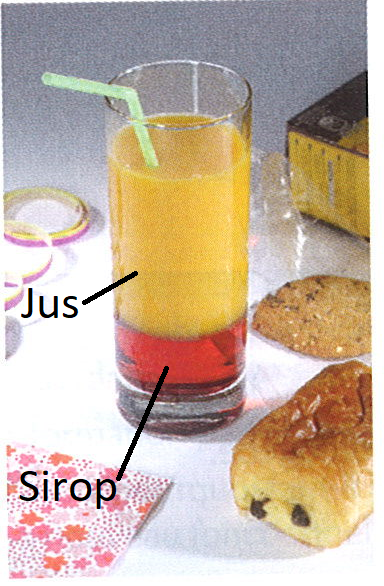
\includegraphics[scale=0.4]{img/jus}
	\end{center}
\end{multicols}